\documentclass{beamer}

% Should be documentclass beamer

\mode<presentation>
{
%  \usetheme[hideothersubsections]{PaloAlto}
  \usetheme{metropolis}
  \setbeamercovered{transparent}
}

\usepackage{amsfonts}
\usepackage{amsmath}
\usepackage{amssymb}
\usepackage{color}
\usepackage{tikz}
\usepackage{pgfplots}
\usepackage{listings}
\usepackage{courier}
%\usepackage[utf8]{inputenc}
%\usepackage[russian]{babel}

\lstset{
  numbers=left,
  basicstyle=\ttfamily\footnotesize,
  numberstyle=\tiny\color{gray},
  stepnumber=1,
  numbersep=10pt,
}

\newcommand{\iu}{\ensuremath{\mathrm{i}}}
\newcommand{\bbR}{\mathbb{R}}
\newcommand{\bbC}{\mathbb{C}}
\newcommand{\calV}{\mathcal{V}}
\newcommand{\calW}{\mathcal{W}}
\newcommand{\macheps}{\epsilon_{\mathrm{mach}}}
\newcommand{\matlab}{\textsc{Matlab}}

\newcommand{\ddiag}{\operatorname{diag}}
\newcommand{\fl}{\operatorname{fl}}
\newcommand{\nnz}{\operatorname{nnz}}
\newcommand{\tr}{\operatorname{tr}}
\renewcommand{\vec}{\operatorname{vec}}

\newcommand{\vertiii}[1]{{\left\vert\kern-0.25ex\left\vert\kern-0.25ex\left\vert #1
    \right\vert\kern-0.25ex\right\vert\kern-0.25ex\right\vert}}
\newcommand{\ip}[2]{\langle #1, #2 \rangle}
\newcommand{\ipx}[2]{\left\langle #1, #2 \right\rangle}
\newcommand{\order}[1]{O( #1 )}

\newcommand{\kron}{\otimes}


\newcommand{\hdr}[2]{
  \title[CS 5220, Fall 2017]{CS 5220: #2}
  \author{David Bindel}
  \date{#1}
}

\newcommand{\calK}{\mathcal{K}}

\hdr{2017-10-26}{More Sparse LA}

\begin{document}

\begin{frame}
  \titlepage
\end{frame}


\begin{frame}
  \frametitle{Reminder: Conjugate Gradients}

  What if we only know how to multiply by $A$? \\
  About all you can do is keep multiplying!
  \[
    \calK_k(A,b) = \operatorname{span}\left\{ 
      b, A b, A^2 b, \ldots, A^{k-1} b \right\}.
  \]
  Gives surprisingly useful information!

  \vspace{5mm}
  If $A$ is symmetric and positive definite,
  $x = A^{-1}b$ minimizes
  \begin{align*}
    \phi(x) &= \frac{1}{2} x^T A x - x^T  b\\
    \nabla \phi(x) &= Ax - b.
  \end{align*}
  Idea: Minimize $\phi(x)$ over $\calK_k(A,b)$. \\
  Basis for the {\em method of conjugate gradients}
\end{frame}


\begin{frame}
  \frametitle{Convergence of CG}

  \begin{itemize}
  \item KSPs are {\em not} stationary (no constant fixed-point iteration)
  \item Convergence is surprisingly subtle!
  \item CG convergence upper bound via {\em condition number}
    \begin{itemize}
    \item Large condition number iff form $\phi(x)$ has long narrow bowl
    \item Usually happens for Poisson and related problems
    \end{itemize}
  \item {\em Preconditioned} problem
    $M^{-1} A x = M^{-1} b$ converges faster?
  \item Whence $M$?  
    \begin{itemize}
    \item From a stationary method?
    \item From a simpler/coarser discretization?
    \item From approximate factorization?
    \end{itemize}
  \end{itemize}
\end{frame}


\begin{frame}[fragile]
  \frametitle{PCG}

\begin{minipage}{0.6\textwidth}
\begin{tabbing}
Compute $r^{(0)} = b - Ax$ \\
for \= $i = 1, 2, \ldots$ \\
\> solve $Mz^{(i-1)} = r^{(i-1)}$ \\
\> $\rho_{i-1} = (r^{(i-1)})^T z^{(i-1)}$ \\
\> if \= $i == 1$ \\
\> \> $p^{(1)} = z^{(0)}$ \\
\> else \\
\> \> $\beta_{i-1} = \rho_{i-1}/\rho_{i-2}$ \\
\> \> $p^{(i)} = z^{(i-1)} + \beta_{i-1} p^{(i-1)}$ \\
\> endif \\
\> $q^{(i)} = A p^{(i)}$ \\
\> $\alpha_i = \rho_{i-1} / (p^{(i)})^T q^{(i)}$ \\
\> $x^{(i)} = x^{(i-1)} + \alpha_i p^{(i)}$ \\
\> $r^{(i)} = r^{(i-1)} - \alpha_i q^{(i)}$ \\
end
\end{tabbing}
\end{minipage}
\begin{minipage}{0.35\textwidth}
  Parallel work:
  \begin{itemize}
    \item Solve with $M$
    \item Product with $A$
    \item Dot products
    \item Axpys
  \end{itemize}
  Overlap comm/comp.
\end{minipage}

\end{frame}


\begin{frame}[fragile]
  \frametitle{PCG bottlenecks}

  Key: fast solve with $M$, product with $A$
  \begin{itemize}
  \item Some preconditioners parallelize better! \\
    (Jacobi vs Gauss-Seidel)
  \item Balance speed with performance.
    \begin{itemize}
    \item Speed for set up of $M$?
    \item Speed to apply $M$ after setup?
    \end{itemize}
  \item Cheaper to do two multiplies/solves at once...
    \begin{itemize}
    \item Can't exploit in obvious way --- lose stability
    \item Variants allow multiple products --- Hoemmen's thesis
    \end{itemize}
  \item Lots of fiddling possible with $M$; what about
    matvec with $A$?
  \end{itemize}

\end{frame}


\begin{frame}
  \frametitle{Thinking on (basic) CG convergence}

  \begin{center}
    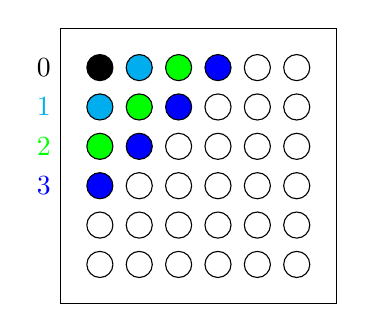
\begin{tikzpicture}
  \draw (0,0) rectangle (3.5,3.5);
  \node at (0,3.0) [left] {0};
  \node at (0,2.5) [left] {\color{cyan}{1}};
  \node at (0,2.0) [left] {\color{green}{2}};
  \node at (0,1.5) [left] {\color{blue}{3}};
  
  \node[circle,draw=black] at (0.5,0.5) {};
  \node[circle,draw=black] at (1.0,0.5) {};
  \node[circle,draw=black] at (1.5,0.5) {};
  \node[circle,draw=black] at (2.0,0.5) {};
  \node[circle,draw=black] at (2.5,0.5) {};
  \node[circle,draw=black] at (3.0,0.5) {};

  \node[circle,draw=black] at (0.5,1.0) {};
  \node[circle,draw=black] at (1.0,1.0) {};
  \node[circle,draw=black] at (1.5,1.0) {};
  \node[circle,draw=black] at (2.0,1.0) {};
  \node[circle,draw=black] at (2.5,1.0) {};
  \node[circle,draw=black] at (3.0,1.0) {};

  \node[circle,draw=black,fill=blue] at (0.5,1.5) {};
  \node[circle,draw=black] at (1.0,1.5) {};
  \node[circle,draw=black] at (1.5,1.5) {};
  \node[circle,draw=black] at (2.0,1.5) {};
  \node[circle,draw=black] at (2.5,1.5) {};
  \node[circle,draw=black] at (3.0,1.5) {};

  \node[circle,draw=black,fill=green] at (0.5,2.0) {};
  \node[circle,draw=black,fill=blue ] at (1.0,2.0) {};
  \node[circle,draw=black] at (1.5,2.0) {};
  \node[circle,draw=black] at (2.0,2.0) {};
  \node[circle,draw=black] at (2.5,2.0) {};
  \node[circle,draw=black] at (3.0,2.0) {};

  \node[circle,draw=black,fill=cyan ] at (0.5,2.5) {};
  \node[circle,draw=black,fill=green] at (1.0,2.5) {};
  \node[circle,draw=black,fill=blue ] at (1.5,2.5) {};
  \node[circle,draw=black] at (2.0,2.5) {};
  \node[circle,draw=black] at (2.5,2.5) {};
  \node[circle,draw=black] at (3.0,2.5) {};

  \node[circle,draw=black,fill=black] at (0.5,3.0) {};
  \node[circle,draw=black,fill=cyan ] at (1.0,3.0) {};
  \node[circle,draw=black,fill=green] at (1.5,3.0) {};
  \node[circle,draw=black,fill=blue ] at (2.0,3.0) {};
  \node[circle,draw=black] at (2.5,3.0) {};
  \node[circle,draw=black] at (3.0,3.0) {};

\end{tikzpicture}

  \end{center}
  Consider 2D Poisson with 5-point stencil on an $n \times n$ mesh.
  \begin{itemize}
  \item Information moves one grid cell per matvec.
  \item Cost per matvec is $O(n^2)$.
  \item At least $O(n^3)$ work to get information across mesh!
  \end{itemize}
\end{frame}


\begin{frame}
  \frametitle{CG convergence: a counting approach}

  \begin{itemize}
  \item Time to converge $\geq$ time to propagate info across mesh
  \item For a 2D mesh: $O(n)$ matvecs, $O(n^3) = O(N^{3/2})$ cost
  \item For a 3D mesh: $O(n)$ matvecs, $O(n^4) = O(N^{4/3})$ cost
  \item ``Long'' meshes yield slow convergence
  \item 3D beats 2D because everything is closer!
    \begin{itemize}
    \item Advice: sparse direct for 2D, CG for 3D.
    \item Better advice: use a preconditioner!
    \end{itemize}
  \end{itemize}
\end{frame}


\begin{frame}
  \frametitle{CG convergence: an eigenvalue approach}

  Define the {\em condition number} for $\kappa(L)$ s.p.d:
  \[
    \kappa(L) = \frac{\lambda_{\max}(L)}{\lambda_{\min}(L)}
  \]
  Describes how elongated the level surfaces of $\phi$ are.

  \vspace{5mm}
  \begin{itemize}
  \item
    For Poisson, $\kappa(L) = O(h^{-2})$
  \item
    CG steps to reduce error by $1/2$ = 
    $O(\sqrt{\kappa}) = O(h^{-1})$.
  \end{itemize}
  
  \vspace{5mm}
  Similar back-of-the-envelope estimates for some other PDEs.
  But these are not always that useful... can be pessimistic
  if there are only a few extreme eigenvalues.
\end{frame}


\begin{frame}
  \frametitle{CG convergence: a frequency-domain approach}

  \begin{tabular}{cc}
    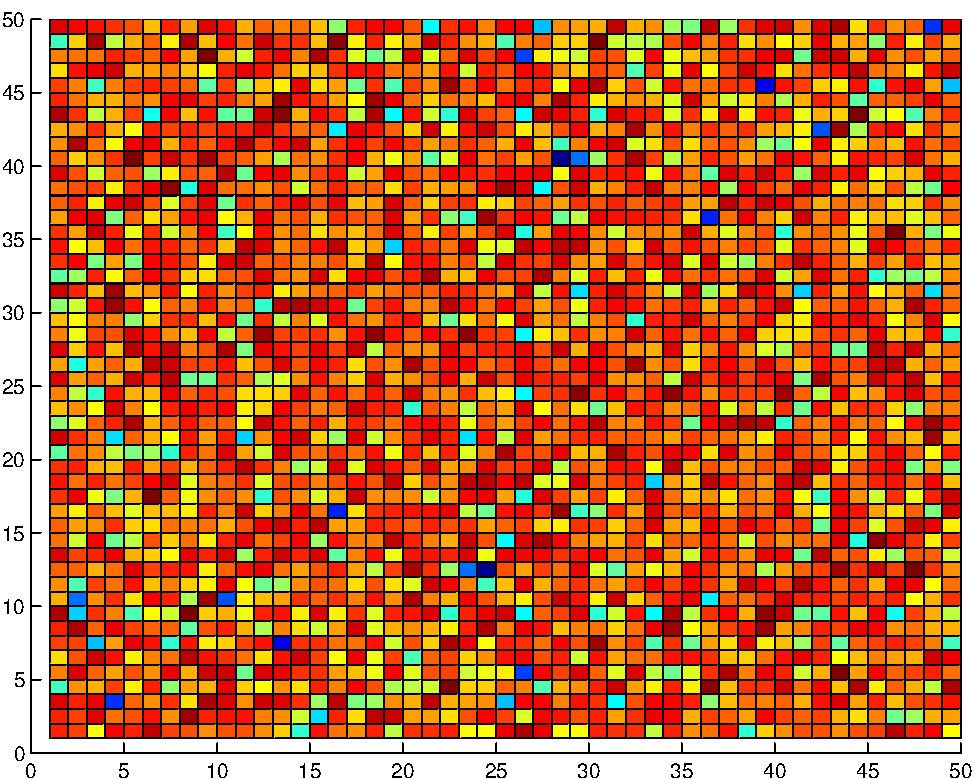
\includegraphics[width=0.48\textwidth]{figs/cg1init.pdf} &
    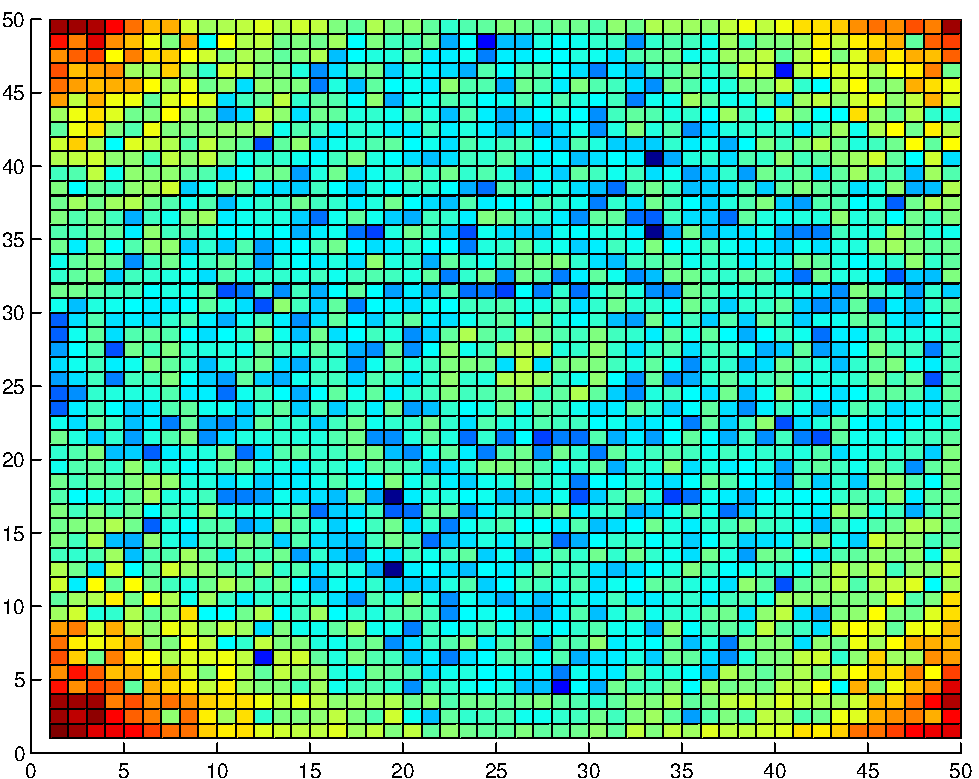
\includegraphics[width=0.48\textwidth]{figs/cg1swept.pdf} \\
    FFT of $e_0$ & FFT of $e_{10}$
  \end{tabular}

  \begin{center}
  Error $e_k$ after $k$ steps of CG gets smoother!
  \end{center}
\end{frame}


\begin{frame}
  \frametitle{Choosing preconditioners for 2D Poisson}

  \begin{itemize}
  \item CG already handles high-frequency error
  \item Want something to deal with lower frequency!
  \item Jacobi useless
    \begin{itemize}
    \item Doesn't even change Krylov subspace!
    \end{itemize}
  \item Better idea: block Jacobi?
    \begin{itemize}
    \item Q: How should things split up?
    \item A: Minimize blocks across domain.
    \item Compatible with minimizing communication!
    \end{itemize}
  \end{itemize}
\end{frame}


\begin{frame}
  \frametitle{Restrictive Additive Schwartz (RAS)}

  \begin{center}
    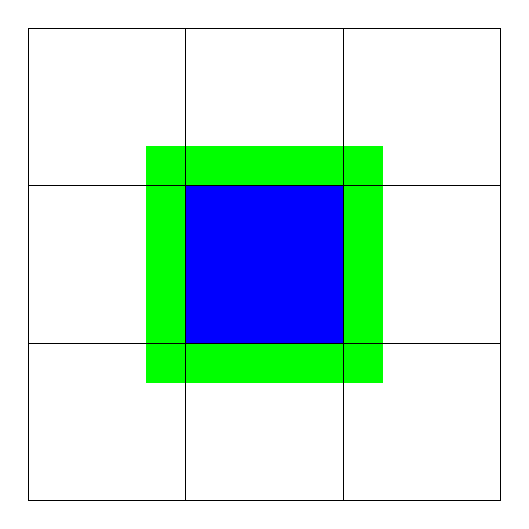
\begin{tikzpicture}[scale=2]
      \draw[draw=green,fill=green] (0.75,0.75) rectangle (2.25,2.25);
      \draw[fill=blue] (1,1) rectangle (2,2);
      \draw[step=1] (0,0) grid (3,3);
    \end{tikzpicture}
  \end{center}
\end{frame}


\begin{frame}
  \frametitle{Restrictive Additive Schwartz (RAS)}

  \begin{center}
    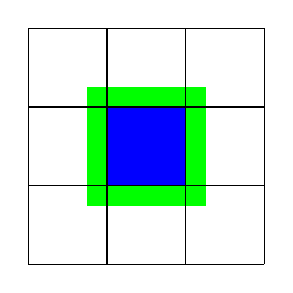
\begin{tikzpicture}
      \draw[draw=green,fill=green] (0.75,0.75) rectangle (2.25,2.25);
      \draw[fill=blue] (1,1) rectangle (2,2);
      \draw[step=1] (0,0) grid (3,3);
    \end{tikzpicture}
  \end{center}

  \begin{itemize}
  \item Get {\color{green} ghost cell data}
  \item Solve {\em everything} local (including neighbor data)
  \item Update {\color{blue} local values} for next step
  \item Default strategy in PETSc
  \end{itemize}
\end{frame}


\begin{frame}
  \frametitle{Multilevel Ideas}

  \begin{itemize}
  \item RAS propogates information by one processor per step
  \item For scalability, still need to get around this!
  \item Basic idea: use multiple grids
    \begin{itemize}
    \item Fine grid gives lots of work, kills high-freq error
    \item Coarse grid cheaply gets info across mesh, kills low freq
    \end{itemize}
  \end{itemize}
  More on this another time.
\end{frame}


\begin{frame}
  \frametitle{CG performance}
  
  Two ways to get better performance from CG:
  \begin{enumerate}
  \item Better preconditioner 
    \begin{itemize}
    \item Improves asymptotic complexity?
    \item ... but application dependent
    \end{itemize}
  \item Tuned implementation
    \begin{itemize}
    \item Improves constant in big-O
    \item ... but application independent?
    \end{itemize}
  \end{enumerate}
  Benchmark idea (?): no preconditioner, just tune.
  
\end{frame}


\begin{frame}[fragile]
  \frametitle{Tuning PCG}

\begin{minipage}{0.5\textwidth}
\begin{tabbing}
Compute $r^{(0)} = b - Ax$ \\
for \= $i = 1, 2, \ldots$ \\
\> solve $Mz^{(i-1)} = r^{(i-1)}$ \\
\> $\rho_{i-1} = (r^{(i-1)})^T z^{(i-1)}$ \\
\> if \= $i == 1$ \\
\> \> $p^{(1)} = z^{(0)}$ \\
\> else \\
\> \> $\beta_{i-1} = \rho_{i-1}/\rho_{i-2}$ \\
\> \> $p^{(i)} = z^{(i-1)} + \beta_{i-1} p^{(i-1)}$ \\
\> endif \\
\> $q^{(i)} = A p^{(i)}$ \\
\> $\alpha_i = \rho_{i-1} / (p^{(i)})^T q^{(i)}$ \\
\> $x^{(i)} = x^{(i-1)} + \alpha_i p^{(i)}$ \\
\> $r^{(i)} = r^{(i-1)} - \alpha_i q^{(i)}$ \\
end
\end{tabbing}
\end{minipage}
\begin{minipage}{0.45\textwidth}
  \begin{itemize}
  \item Most work in $A$, $M$
  \item Vector ops synchronize
  \item Overlap comm, comp?
  \end{itemize}
\end{minipage}

\end{frame}


\begin{frame}[fragile]
  \frametitle{Tuning PCG}

\begin{minipage}{0.5\textwidth}
\begin{tabbing}
Compute $r^{(0)} = b - Ax$ \\
$p_{-1} = 0; \beta_{-1} = 0; \alpha_{-1} = 0$ \\
$s = L^{-1} r^{(0)}$ \\
$\rho_0 = s^T s$ \\
for \= $i = 0, 1, 2, \ldots$ \\
\> $w_i = L^{-T} s$ \\
\> $p_i = w_i + \beta_{i-1} p_{i-1}$ \\
\> $q_i = A p_i$ \\
\> $\gamma = p_i^T q_i$ \\
\> $x_i = x_{i-1} + \alpha_{i-1} p_{i-1}$ \\
\> $\alpha_{i} = \rho_{i}/\gamma_{i}$ \\
\> $r_{i+1} = r_i - \alpha q_{i}$ \\
\> $s = L^{-1} r_{i+1}$ \\
\> $\rho_{i+1} = s^T s$ \\
\> Check convergence ($\|r_{i+1}\|$) \\
\> $\beta_{i} = \rho_{i+1}/\rho_i$ \\
end
\end{tabbing}
\end{minipage}
\begin{minipage}{0.5\textwidth}
  Split $z = M^{-1} r$ into $s, w_i$ \\
  Overlap
  \begin{itemize}
  \item $p_i^T q_i$ with $x$ update
  \item $s^T s$ with $w_i$ eval
  \item Computing $p_i$, $q_i$, $\gamma$
  \item Pipeline $r_{i+1}$, $s$?
  \item Pipeline $p_i$, $w_i$?
  \end{itemize}

  \vspace{5mm}
  Parallel Numerical LA, \\
  Demmel, Heath, van der Vorst
\end{minipage}

\end{frame}


\begin{frame}[fragile]
  \frametitle{Tuning PCG}
  
  Can also tune
  \begin{itemize}
  \item Preconditioner solve (hooray!)
  \item Matrix multiply
    \begin{itemize}
    \item Represented implicitly (regular grids)
    \item Or explicitly (e.g. compressed sparse column)
    \end{itemize}
  \end{itemize}
  Or further rearrange algorithm (Hoemmen, Demmel).
\end{frame}

\begin{frame}
  \frametitle{Tuning sparse matvec}

  \begin{itemize}
  \item Sparse matrix blocking and reordering (Im, Vuduc, Yelick)
    \begin{itemize}
    \item Packages: Sparsity (Im), OSKI (Vuduc)
    \item Available as PETSc extension
    \end{itemize}
  \item Optimizing stencil operations (Datta)
  \end{itemize}
\end{frame}


\begin{frame}[fragile]
  \frametitle{Reminder: Compressed sparse row storage}

  \begin{center}
    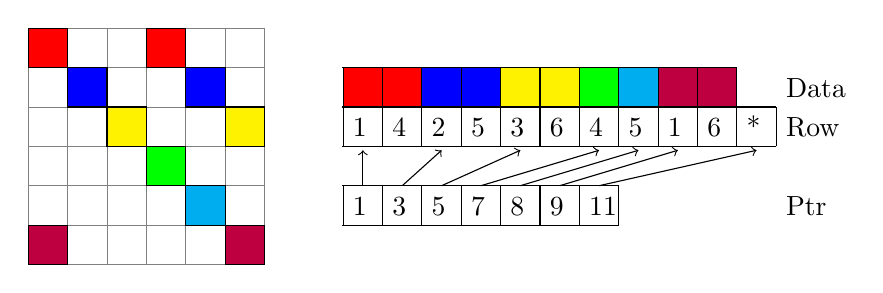
\begin{tikzpicture}
  \draw[step=0.5,gray,very thin] (-1,0) grid (2.0,3.0);
  \draw[fill=red]    (-1.0,2.5) rectangle (-0.5,3.0);
  \draw[fill=red]    ( 0.5,2.5) rectangle ( 1.0,3.0);
  \draw[fill=blue]   (-0.5,2.0) rectangle ( 0.0,2.5);
  \draw[fill=blue]   ( 1.0,2.0) rectangle ( 1.5,2.5);
  \draw[fill=yellow] ( 0.0,1.5) rectangle ( 0.5,2.0);
  \draw[fill=yellow] ( 1.5,1.5) rectangle ( 2.0,2.0);
  \draw[fill=green]  ( 0.5,1.0) rectangle ( 1.0,1.5);
  \draw[fill=cyan]   ( 1.0,0.5) rectangle ( 1.5,1.0);
  \draw[fill=purple] ( 1.5,0.0) rectangle ( 2.0,0.5);
  \draw[fill=purple] (-1.0,0.0) rectangle (-0.5,0.5);

  \draw[fill=red]    (3.0,2.0) rectangle (4.0,2.5);
  \draw[fill=blue]   (4.0,2.0) rectangle (5.0,2.5);
  \draw[fill=yellow] (5.0,2.0) rectangle (6.0,2.5);
  \draw[fill=green]  (6.0,2.0) rectangle (6.5,2.5);
  \draw[fill=cyan]   (6.5,2.0) rectangle (7.0,2.5);
  \draw[fill=purple] (7.0,2.0) rectangle (8.0,2.5);
  
  \draw[step=0.5,black] (2.99,2.0) grid (8.0,2.5);
  \draw[step=0.5,black] (2.99,1.499) grid (8.5,2.0);
  \draw[step=0.5,black] (2.99,0.499) grid (6.5,1.0);

  \draw (3.0,1.5) node[anchor=south west] {1};
  \draw (3.5,1.5) node[anchor=south west] {4};
  \draw (4.0,1.5) node[anchor=south west] {2};
  \draw (4.5,1.5) node[anchor=south west] {5};
  \draw (5.0,1.5) node[anchor=south west] {3};
  \draw (5.5,1.5) node[anchor=south west] {6};
  \draw (6.0,1.5) node[anchor=south west] {4};
  \draw (6.5,1.5) node[anchor=south west] {5};
  \draw (7.0,1.5) node[anchor=south west] {1};
  \draw (7.5,1.5) node[anchor=south west] {6};
  \draw (8.0,1.5) node[anchor=south west] {*};

  \draw (3.0,0.5) node[anchor=south west] {1};
  \draw (3.5,0.5) node[anchor=south west] {3};
  \draw (4.0,0.5) node[anchor=south west] {5};
  \draw (4.5,0.5) node[anchor=south west] {7};
  \draw (5.0,0.5) node[anchor=south west] {8};
  \draw (5.5,0.5) node[anchor=south west] {9};
  \draw (6.0,0.5) node[anchor=south west] {11};

  \draw [->] (3.25,1.0) -- (3.25,1.45); % 1
  \draw [->] (3.75,1.0) -- (4.25,1.45); % 3
  \draw [->] (4.25,1.0) -- (5.25,1.45); % 5
  \draw [->] (4.75,1.0) -- (6.25,1.45); % 7
  \draw [->] (5.25,1.0) -- (6.75,1.45); % 8
  \draw [->] (5.75,1.0) -- (7.25,1.45); % 9
  \draw [->] (6.25,1.0) -- (8.25,1.45);

  \draw (8.5,2.0) node[anchor=south west] {Data};
  \draw (8.5,1.5) node[anchor=south west] {Row};
  \draw (8.5,0.5) node[anchor=south west] {Ptr};
\end{tikzpicture}

  \end{center}

\begin{lstlisting}
for i = 1:n
  y[i] = 0;
  for jj = ptr[i] to ptr[i+1]-1
    y[i] += A[jj]*x[col[j]];
  end
end
\end{lstlisting}
Problem: {\tt y[i] += A[jj]*x[{\bf \color{red}col[j]}];}

\end{frame}


\begin{frame}
  \frametitle{Memory traffic in CSR multiply}

  Memory access patterns:
  \begin{itemize}
  \item Elements of $y$ accessed sequentially
  \item Elements of $A$ accessed sequentially
  \item Access to $x$ are all over!
  \end{itemize}
  Can help by switching to block CSR. \\
  Switching to single precision, short indices can help 
  memory traffic, too!
\end{frame}


\begin{frame}
  \frametitle{Parallelizing matvec}

  %  \includegraphics{lec15pspmv.pdf}
  \begin{center}
    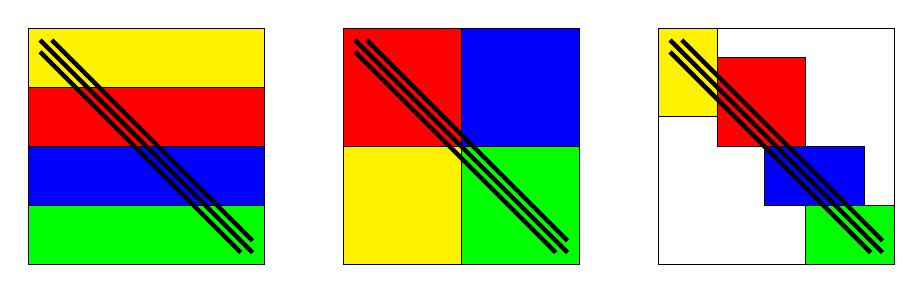
\begin{tikzpicture}
      \begin{scope}[scale=0.75]
        \draw[fill=yellow] (0,4) rectangle (4,3);
        \draw[fill=red]    (0,3) rectangle (4,2);
        \draw[fill=blue]   (0,2) rectangle (4,1);
        \draw[fill=green]  (0,1) rectangle (4,0);
        \draw[ultra thick] (0.2,3.8) -- (3.8,0.2);
        \draw[ultra thick] (0.4,3.8) -- (3.8,0.4);
        \draw[ultra thick] (0.2,3.6) -- (3.6,0.2);
      \end{scope}
      \begin{scope}[xshift=4cm,scale=0.75]
        \draw[fill=yellow] (0,0) rectangle (2,2);
        \draw[fill=red]    (0,2) rectangle (2,4);
        \draw[fill=blue]   (2,2) rectangle (4,4);
        \draw[fill=green]  (2,0) rectangle (4,2);
        \draw[ultra thick] (0.2,3.8) -- (3.8,0.2);
        \draw[ultra thick] (0.4,3.8) -- (3.8,0.4);
        \draw[ultra thick] (0.2,3.6) -- (3.6,0.2);
      \end{scope}
      \begin{scope}[xshift=8cm,scale=0.75]
        \draw (0,0) rectangle (4,4);
        \draw[fill=yellow] (0,4) rectangle (1,2.5);
        \draw[fill=red]    (1,3.5) rectangle (2.5,2);
        \draw[fill=blue]   (1.8,2) rectangle (3.5,1);
        \draw[fill=green]  (2.5,1) rectangle (4,0);
        \draw[ultra thick] (0.2,3.8) -- (3.8,0.2);
        \draw[ultra thick] (0.4,3.8) -- (3.8,0.4);
        \draw[ultra thick] (0.2,3.6) -- (3.6,0.2);
      \end{scope}
    \end{tikzpicture}
  \end{center}
  \begin{itemize}
  \item Each processor gets a piece
  \item Many partitioning strategies
  \item Idea: re-order so one of these strategies is ``good''
  \end{itemize}

\end{frame}


\begin{frame}
  \frametitle{Reordering for matvec}

  SpMV performance goals:
  \begin{itemize}
  \item Balance load?
  \item Balance storage?
  \item Minimize communication?
  \item Good cache re-use?
  \end{itemize}
  Also reorder for 
  \begin{itemize}
  \item Stability of Gauss elimination,
  \item Fill reduction in Gaussian elimination,
  \item Improved performance of preconditioners...
  \end{itemize}

\end{frame}


\begin{frame}
  \frametitle{Reminder: Sparsity and partitioning}

  \begin{center}
    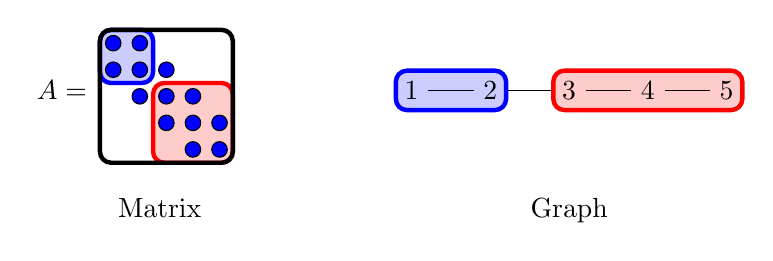
\begin{tikzpicture}

      % A = spy plot
      \draw (0,0.75) node[anchor=east] {$A=$};
      \begin{scope}[xshift=6pt,scale=2]
        \draw[ultra thick,rounded corners,color=blue,fill=blue!20] (-2.40pt,12.00pt) rectangle
        (7.20pt,21.60pt);
        \draw[ultra thick,rounded corners,color=red,fill=red!20]
        (7.20pt,12.00pt) rectangle
        (21.60pt,-2.40pt);

        \draw[ultra thick,rounded corners] (-2.40pt,21.60pt) rectangle (21.60pt,-2.40pt);
\draw[fill=blue] (0.00pt,19.20pt) circle [radius=1.4pt]; 
\draw[fill=blue] (4.80pt,19.20pt) circle [radius=1.4pt]; 
\draw[fill=blue] (0.00pt,14.40pt) circle [radius=1.4pt]; 
\draw[fill=blue] (4.80pt,14.40pt) circle [radius=1.4pt]; 
\draw[fill=blue] (9.60pt,14.40pt) circle [radius=1.4pt]; 
\draw[fill=blue] (4.80pt,9.60pt) circle [radius=1.4pt]; 
\draw[fill=blue] (9.60pt,9.60pt) circle [radius=1.4pt]; 
\draw[fill=blue] (14.40pt,9.60pt) circle [radius=1.4pt]; 
\draw[fill=blue] (9.60pt,4.80pt) circle [radius=1.4pt]; 
\draw[fill=blue] (14.40pt,4.80pt) circle [radius=1.4pt]; 
\draw[fill=blue] (19.20pt,4.80pt) circle [radius=1.4pt]; 
\draw[fill=blue] (14.40pt,0.00pt) circle [radius=1.4pt]; 
\draw[fill=blue] (19.20pt,0.00pt) circle [radius=1.4pt]; 

      \end{scope}

      % Graph picture
      \begin{scope}[xshift=4cm]
        \draw[ultra thick,rounded corners,color=blue,fill=blue!20]
          (-0.2,0.5) rectangle (1.2,1);
        \draw[ultra thick,rounded corners,color=red,fill=red!20]
          (1.8,0.5) rectangle (4.2,1);
        \node (A) at (0,0.75) {1};
        \node (B) at (1,0.75) {2};
        \node (C) at (2,0.75) {3};
        \node (D) at (3,0.75) {4};
        \node (E) at (4,0.75) {5};
        \draw (A) -- (B) -- (C) -- (D) -- (E);
      \end{scope}

      \node[anchor=north] at (0.8,-0.5) {Matrix};
      \node[anchor=north] at (6,-0.5) {Graph};
    \end{tikzpicture}
  \end{center}

  Want to partition sparse graphs so that
  \begin{itemize}
  \item Subgraphs are same size (load balance)
  \item Cut size is minimal (minimize communication)
  \end{itemize}
  Matrices that are ``almost'' diagonal are good?

\end{frame}


\begin{frame}
  \frametitle{Reordering for bandedness}

  \begin{tabular}{cc}
  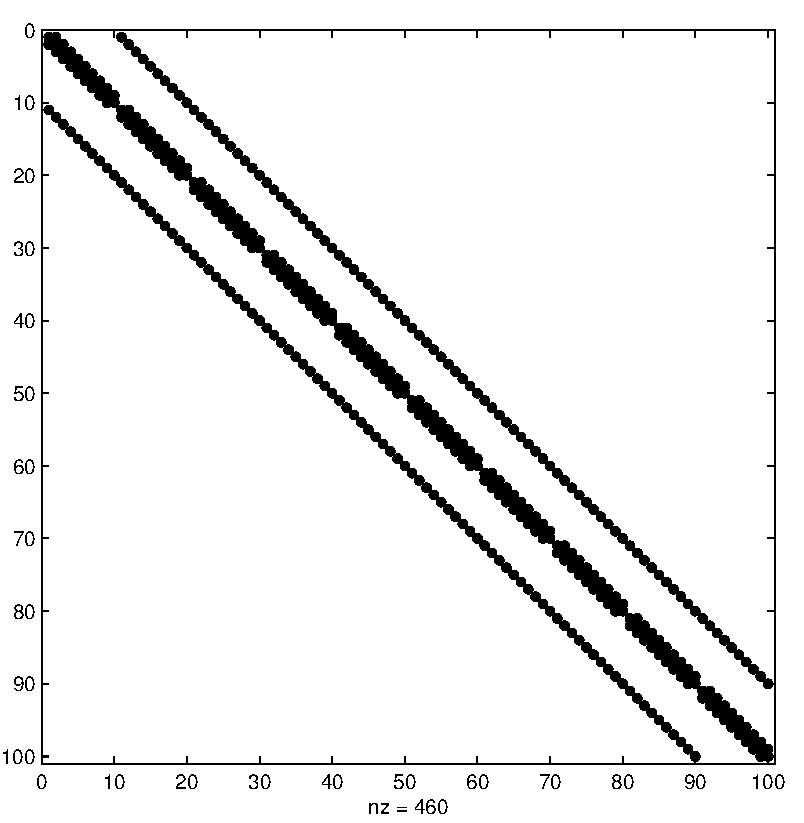
\includegraphics[width=0.42\textwidth]{figs/laplace2d-spy.pdf} &
  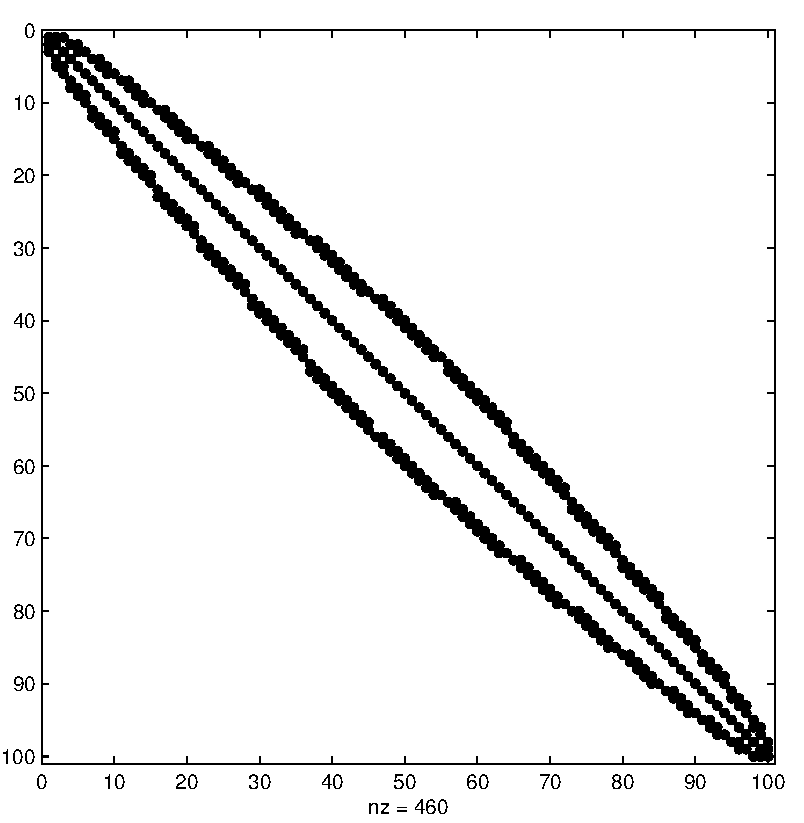
\includegraphics[width=0.42\textwidth]{figs/laplace2d-spy-rcm.pdf} \\
  Natural order & RCM reordering
  \end{tabular}
  
  \vspace{1mm}
  Reverse Cuthill-McKee
  \begin{itemize}
  \item Select ``peripheral'' vertex $v$
  \item Order according to breadth first search from $v$
  \item Reverse ordering
  \end{itemize}
\end{frame}

\begin{frame}
  \frametitle{From iterative to direct}
  
  \begin{itemize}
  \item RCM ordering is great for SpMV
  \item But isn't narrow banding good for solvers, too?
    \begin{itemize}
    \item LU takes $O(nb^2)$ where $b$ is bandwidth.
    \item Great if there's an ordering where $b$ is small!
    \end{itemize}
  \end{itemize}
\end{frame}


\begin{frame}
  \frametitle{Skylines and profiles}

  \begin{itemize}
  \item {\em Profile} solvers generalize band solvers
  \item Skyline storage for storing lower triangle: for each row $i$,
    \begin{itemize}
    \item Start and end of storage for nonzeros in row.
    \item {\em Contiguous} nonzero list up to main diagonal.
    \end{itemize}
  \item In each column, first nonzero defines a profile.
  \item All fill-in confined to profile.
  \item RCM is again a good ordering.
  \end{itemize}
\end{frame}


\begin{frame}
  \frametitle{Beyond bandedness}

  \begin{itemize}
  \item Bandedness only takes us so far
    \begin{itemize}
    \item Minimum bandwidth for 2D model problem?  3D?
    \item Skyline only gets us so much farther
    \end{itemize}
  \item But more general solvers have similar structure
    \begin{itemize}
    \item Ordering (minimize fill)
    \item Symbolic factorization (where will fill be?)
    \item Numerical factorization (pivoting?)
    \item ... and triangular solves
    \end{itemize}
  \end{itemize}
\end{frame}


\begin{frame}
  \frametitle{Reminder: Matrices to graphs}

  \begin{itemize}
  \item $A_{ij} \neq 0$ means there is an edge between $i$ and $j$
  \item Ignore self-loops and weights for the moment
  \item Symmetric matrices correspond to undirected graphs
  \end{itemize}
\end{frame}


\begin{frame}
  \frametitle{Troublesome Trees}

  \begin{center}
    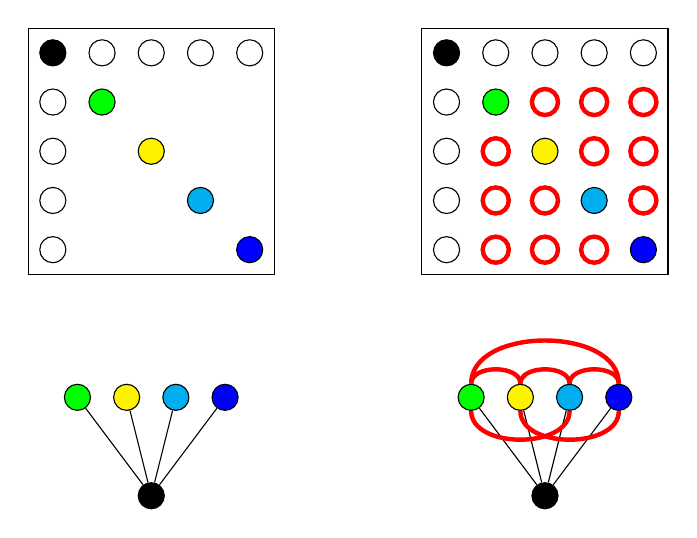
\begin{tikzpicture}[scale=1.25]
      \begin{scope}
        \draw (0.25,0.25) rectangle (2.75,2.75);
        \node at (0.5,2.0) [circle,draw=black] {};
        \node at (0.5,1.5) [circle,draw=black] {};
        \node at (0.5,1.0) [circle,draw=black] {};
        \node at (0.5,0.5) [circle,draw=black] {};
        \node at (1.0,2.5) [circle,draw=black] {};
        \node at (1.5,2.5) [circle,draw=black] {};
        \node at (2.0,2.5) [circle,draw=black] {};
        \node at (2.5,2.5) [circle,draw=black] {};
        \node at (0.5,2.5) [circle,draw=black,fill=black] {};      
        \node at (1.0,2.0) [circle,draw=black,fill=green] {};
        \node at (1.5,1.5) [circle,draw=black,fill=yellow] {};
        \node at (2.0,1.0) [circle,draw=black,fill=cyan] {};
        \node at (2.5,0.5) [circle,draw=black,fill=blue] {};
      \end{scope}

      \begin{scope}[yshift=-2cm]
        \node (R0) at (1.5,0) [circle,draw=black,fill=black] {};
        \node (A0) at (0.75,1) [circle,draw=black,fill=green] {};
        \node (B0) at (1.25,1) [circle,draw=black,fill=yellow] {};
        \node (C0) at (1.75,1) [circle,draw=black,fill=cyan] {};
        \node (D0) at (2.25,1) [circle,draw=black,fill=blue] {};
        \draw (R0) -- (A0);
        \draw (R0) -- (B0);
        \draw (R0) -- (C0);
        \draw (R0) -- (D0);
      \end{scope}

      \begin{scope}[xshift=4cm]
        \draw (0.25,0.25) rectangle (2.75,2.75);
        \node at (0.5,2.0) [circle,draw=black] {};
        \node at (0.5,1.5) [circle,draw=black] {};
        \node at (0.5,1.0) [circle,draw=black] {};
        \node at (0.5,0.5) [circle,draw=black] {};
        \node at (1.0,2.5) [circle,draw=black] {};
        \node at (1.5,2.5) [circle,draw=black] {};
        \node at (2.0,2.5) [circle,draw=black] {};
        \node at (2.5,2.5) [circle,draw=black] {};
        \node at (0.5,2.5) [circle,draw=black,fill=black] {};      
        \node at (1.0,2.0) [circle,draw=black,fill=green] {};
        \node at (1.5,1.5) [circle,draw=black,fill=yellow] {};
        \node at (2.0,1.0) [circle,draw=black,fill=cyan] {};
        \node at (2.5,0.5) [circle,draw=black,fill=blue] {};

        \node at (1.0,1.5) [circle,draw=red,ultra thick] {};                
        \node at (1.0,1.0) [circle,draw=red,ultra thick] {};        
        \node at (1.0,0.5) [circle,draw=red,ultra thick] {};
        \node at (1.5,2.0) [circle,draw=red,ultra thick] {};                
        \node at (1.5,1.0) [circle,draw=red,ultra thick] {};        
        \node at (1.5,0.5) [circle,draw=red,ultra thick] {};
        \node at (2.0,2.0) [circle,draw=red,ultra thick] {};                
        \node at (2.0,1.5) [circle,draw=red,ultra thick] {};        
        \node at (2.0,0.5) [circle,draw=red,ultra thick] {};
        \node at (2.5,2.0) [circle,draw=red,ultra thick] {};                
        \node at (2.5,1.5) [circle,draw=red,ultra thick] {};        
        \node at (2.5,1.0) [circle,draw=red,ultra thick] {};
      \end{scope}

      \begin{scope}[xshift=4cm,yshift=-2cm]
        \node (R1) at (1.5,0) [circle,draw=black,fill=black] {};
        \node (A1) at (0.75,1) [circle,draw=black,fill=green] {};
        \node (B1) at (1.25,1) [circle,draw=black,fill=yellow] {};
        \node (C1) at (1.75,1) [circle,draw=black,fill=cyan] {};
        \node (D1) at (2.25,1) [circle,draw=black,fill=blue] {};
        \draw (R1) -- (A1);
        \draw (R1) -- (B1);
        \draw (R1) -- (C1);
        \draw (R1) -- (D1);

        \draw[draw=red,ultra thick] (A1.north) to[out=90,in=90] (B1.north);
        \draw[draw=red,ultra thick] (B1.north) to[out=90,in=90] (C1.north);
        \draw[draw=red,ultra thick] (C1.north) to[out=90,in=90] (D1.north);
        \draw[draw=red,ultra thick] (A1.south) to[out=-90,in=-90] (C1.south);
        \draw[draw=red,ultra thick] (B1.south) to[out=-90,in=-90] (D1.south);
        \draw[draw=red,ultra thick] (A1.north) to[out=90,in=90] (D1.north);
      \end{scope}      
    \end{tikzpicture}
  \end{center}
  One step of Gaussian elimination {\em completely} fills this matrix!
\end{frame}


\begin{frame}
  \frametitle{Terrific Trees}

  \begin{center}
    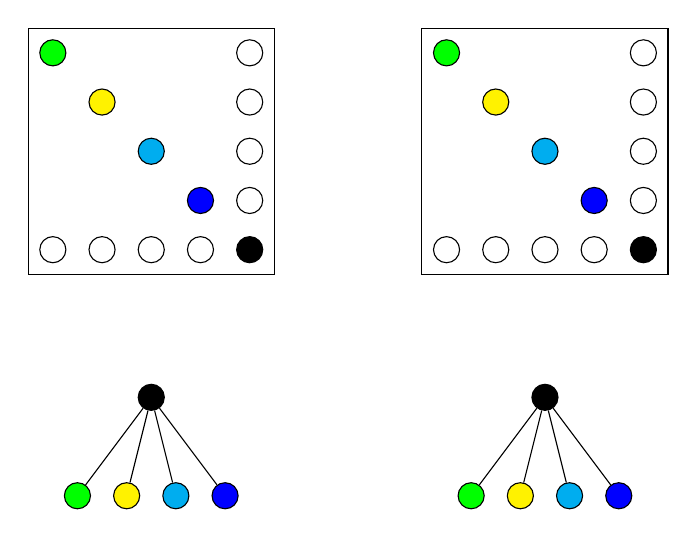
\begin{tikzpicture}[scale=1.25]
      \begin{scope}
        \draw (0.25,0.25) rectangle (2.75,2.75);
        \node at (2.5,2.5) [circle,draw=black] {};
        \node at (2.5,2.0) [circle,draw=black] {};
        \node at (2.5,1.5) [circle,draw=black] {};
        \node at (2.5,1.0) [circle,draw=black] {};
        \node at (0.5,0.5) [circle,draw=black] {};
        \node at (1.0,0.5) [circle,draw=black] {};
        \node at (1.5,0.5) [circle,draw=black] {};
        \node at (2.0,0.5) [circle,draw=black] {};

        \node at (0.5,2.5) [circle,draw=black,fill=green] {};      
        \node at (1.0,2.0) [circle,draw=black,fill=yellow] {};
        \node at (1.5,1.5) [circle,draw=black,fill=cyan] {};
        \node at (2.0,1.0) [circle,draw=black,fill=blue] {};
        \node at (2.5,0.5) [circle,draw=black,fill=black] {};
      \end{scope}

      \begin{scope}[yshift=-2cm]
        \node (R0) at (1.5,1) [circle,draw=black,fill=black] {};
        \node (A0) at (0.75,0) [circle,draw=black,fill=green] {};
        \node (B0) at (1.25,0) [circle,draw=black,fill=yellow] {};
        \node (C0) at (1.75,0) [circle,draw=black,fill=cyan] {};
        \node (D0) at (2.25,0) [circle,draw=black,fill=blue] {};
        \draw (R0) -- (A0);
        \draw (R0) -- (B0);
        \draw (R0) -- (C0);
        \draw (R0) -- (D0);
      \end{scope}

      \begin{scope}[xshift=4cm]
        \draw (0.25,0.25) rectangle (2.75,2.75);
        \node at (2.5,2.5) [circle,draw=black] {};
        \node at (2.5,2.0) [circle,draw=black] {};
        \node at (2.5,1.5) [circle,draw=black] {};
        \node at (2.5,1.0) [circle,draw=black] {};
        \node at (0.5,0.5) [circle,draw=black] {};
        \node at (1.0,0.5) [circle,draw=black] {};
        \node at (1.5,0.5) [circle,draw=black] {};
        \node at (2.0,0.5) [circle,draw=black] {};

        \node at (0.5,2.5) [circle,draw=black,fill=green] {};      
        \node at (1.0,2.0) [circle,draw=black,fill=yellow] {};
        \node at (1.5,1.5) [circle,draw=black,fill=cyan] {};
        \node at (2.0,1.0) [circle,draw=black,fill=blue] {};
        \node at (2.5,0.5) [circle,draw=black,fill=black] {};
      \end{scope}

      \begin{scope}[xshift=4cm,yshift=-2cm]
        \node (R0) at (1.5,1) [circle,draw=black,fill=black] {};
        \node (A0) at (0.75,0) [circle,draw=black,fill=green] {};
        \node (B0) at (1.25,0) [circle,draw=black,fill=yellow] {};
        \node (C0) at (1.75,0) [circle,draw=black,fill=cyan] {};
        \node (D0) at (2.25,0) [circle,draw=black,fill=blue] {};
        \draw (R0) -- (A0);
        \draw (R0) -- (B0);
        \draw (R0) -- (C0);
        \draw (R0) -- (D0);
      \end{scope}

    \end{tikzpicture}
  \end{center}
  Full Gaussian elimination generates {\em no} fill in this matrix!
\end{frame}


\begin{frame}[fragile]
  \frametitle{Graphic Elimination}

  Consider first steps of GE
\begin{lstlisting}
A(2:end,1)     = A(2:end,1)/A(1,1);
A(2:end,2:end) = A(2:end,2:end)-...
                 A(2:end,1)*A(1,2:end);
\end{lstlisting}
  Nonzero in the outer product at $(i,j)$ if {\tt A(i,1)} and {\tt A(j,1)}
  both nonzero --- that is, if $i$ and $j$ are both connected to 1.

\vspace{5mm}
General: Eliminate variable, connect remaining neighbors.

\end{frame}


\begin{frame}
  \frametitle{Terrific Trees Redux}

  \begin{center}
    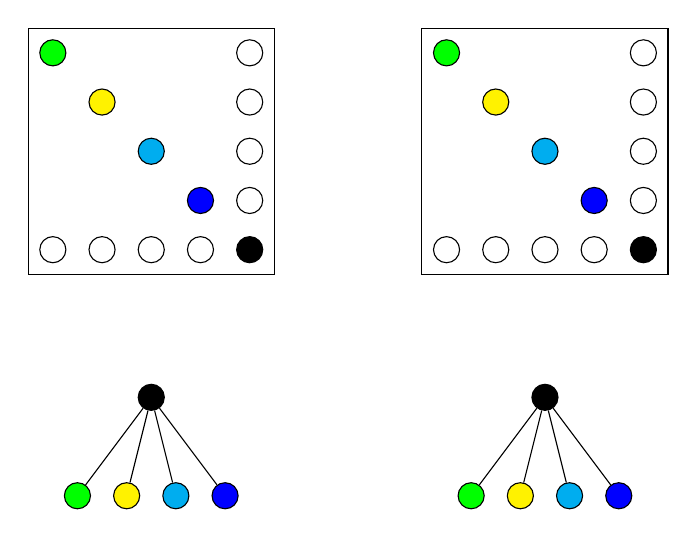
\begin{tikzpicture}[scale=1.25]
      \begin{scope}
        \draw (0.25,0.25) rectangle (2.75,2.75);
        \node at (2.5,2.5) [circle,draw=black] {};
        \node at (2.5,2.0) [circle,draw=black] {};
        \node at (2.5,1.5) [circle,draw=black] {};
        \node at (2.5,1.0) [circle,draw=black] {};
        \node at (0.5,0.5) [circle,draw=black] {};
        \node at (1.0,0.5) [circle,draw=black] {};
        \node at (1.5,0.5) [circle,draw=black] {};
        \node at (2.0,0.5) [circle,draw=black] {};

        \node at (0.5,2.5) [circle,draw=black,fill=green] {};      
        \node at (1.0,2.0) [circle,draw=black,fill=yellow] {};
        \node at (1.5,1.5) [circle,draw=black,fill=cyan] {};
        \node at (2.0,1.0) [circle,draw=black,fill=blue] {};
        \node at (2.5,0.5) [circle,draw=black,fill=black] {};
      \end{scope}

      \begin{scope}[yshift=-2cm]
        \node (R0) at (1.5,1) [circle,draw=black,fill=black] {};
        \node (A0) at (0.75,0) [circle,draw=black,fill=green] {};
        \node (B0) at (1.25,0) [circle,draw=black,fill=yellow] {};
        \node (C0) at (1.75,0) [circle,draw=black,fill=cyan] {};
        \node (D0) at (2.25,0) [circle,draw=black,fill=blue] {};
        \draw (R0) -- (A0);
        \draw (R0) -- (B0);
        \draw (R0) -- (C0);
        \draw (R0) -- (D0);
      \end{scope}

      \begin{scope}[xshift=4cm]
        \draw (0.25,0.25) rectangle (2.75,2.75);
        \node at (2.5,2.5) [circle,draw=black] {};
        \node at (2.5,2.0) [circle,draw=black] {};
        \node at (2.5,1.5) [circle,draw=black] {};
        \node at (2.5,1.0) [circle,draw=black] {};
        \node at (0.5,0.5) [circle,draw=black] {};
        \node at (1.0,0.5) [circle,draw=black] {};
        \node at (1.5,0.5) [circle,draw=black] {};
        \node at (2.0,0.5) [circle,draw=black] {};

        \node at (0.5,2.5) [circle,draw=black,fill=green] {};      
        \node at (1.0,2.0) [circle,draw=black,fill=yellow] {};
        \node at (1.5,1.5) [circle,draw=black,fill=cyan] {};
        \node at (2.0,1.0) [circle,draw=black,fill=blue] {};
        \node at (2.5,0.5) [circle,draw=black,fill=black] {};
      \end{scope}

      \begin{scope}[xshift=4cm,yshift=-2cm]
        \node (R0) at (1.5,1) [circle,draw=black,fill=black] {};
        \node (A0) at (0.75,0) [circle,draw=black,fill=green] {};
        \node (B0) at (1.25,0) [circle,draw=black,fill=yellow] {};
        \node (C0) at (1.75,0) [circle,draw=black,fill=cyan] {};
        \node (D0) at (2.25,0) [circle,draw=black,fill=blue] {};
        \draw (R0) -- (A0);
        \draw (R0) -- (B0);
        \draw (R0) -- (C0);
        \draw (R0) -- (D0);
      \end{scope}

    \end{tikzpicture}
  \end{center}

  Order leaves to root $\implies$ \\
  on eliminating $i$, parent of $i$ is only remaining neighbor.
\end{frame}


\begin{frame}
  \frametitle{Nested Dissection}

  \begin{center}
    %    \includegraphics{lec16ndtree.pdf}
    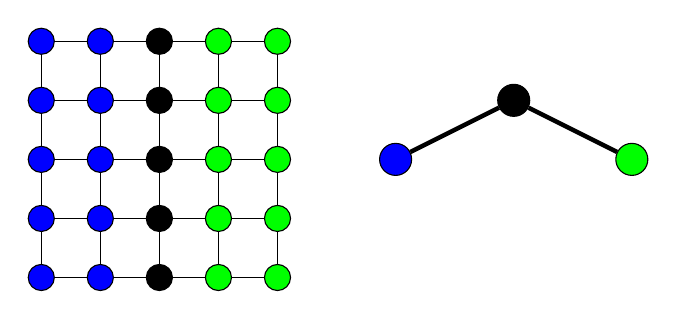
\begin{tikzpicture}[scale=0.75]
      \draw[step=1] (0,0) grid (4,4);
      \node at (0,0) [circle,draw=black,fill=blue] {};
      \node at (0,1) [circle,draw=black,fill=blue] {};
      \node at (0,2) [circle,draw=black,fill=blue] {};
      \node at (0,3) [circle,draw=black,fill=blue] {};
      \node at (0,4) [circle,draw=black,fill=blue] {};
      \node at (1,0) [circle,draw=black,fill=blue] {};
      \node at (1,1) [circle,draw=black,fill=blue] {};
      \node at (1,2) [circle,draw=black,fill=blue] {};
      \node at (1,3) [circle,draw=black,fill=blue] {};
      \node at (1,4) [circle,draw=black,fill=blue] {};
      \node at (2,0) [circle,draw=black,fill=black] {};
      \node at (2,1) [circle,draw=black,fill=black] {};
      \node at (2,2) [circle,draw=black,fill=black] {};
      \node at (2,3) [circle,draw=black,fill=black] {};
      \node at (2,4) [circle,draw=black,fill=black] {};
      \node at (3,0) [circle,draw=black,fill=green] {};
      \node at (3,1) [circle,draw=black,fill=green] {};
      \node at (3,2) [circle,draw=black,fill=green] {};
      \node at (3,3) [circle,draw=black,fill=green] {};
      \node at (3,4) [circle,draw=black,fill=green] {};
      \node at (4,0) [circle,draw=black,fill=green] {};
      \node at (4,1) [circle,draw=black,fill=green] {};
      \node at (4,2) [circle,draw=black,fill=green] {};
      \node at (4,3) [circle,draw=black,fill=green] {};
      \node at (4,4) [circle,draw=black,fill=green] {};

      \node (R1) at (8,3) [circle,draw=black,fill=black] {\;};
      \node (A1) at (6,2) [circle,draw=black,fill=blue] {\;};
      \node (B1) at (10,2) [circle,draw=black,fill=green] {\;};
      \draw[ultra thick] (R1) -- (A1);
      \draw[ultra thick] (R1) -- (B1);
    \end{tikzpicture}
  \end{center}

  \begin{itemize}
  \item Idea: Think of {\em block} tree structures.
  \item Eliminate block trees from bottom up.
  \item Can recursively partition at leaves.
  \item Rough cost estimate: how much just to factor dense Schur 
    complements associated with separators?
  \item Notice graph partitioning appears again!
    \begin{itemize}
    \item And again we want small separators!
    \end{itemize}
  \end{itemize}
\end{frame}


\begin{frame}
  \frametitle{Nested Dissection}

  Model problem: Laplacian with 5 point stencil (for 2D)
  \begin{itemize}
  \item
    ND gives optimal complexity in exact arithmetic \\
    (George 73, Hoffman/Martin/Rose)
  \item 2D: $O(N \log N)$ memory, $O(N^{3/2})$ flops
  \item 3D: $O(N^{4/3})$ memory, $O(N^2)$ flops
  \end{itemize}
\end{frame}

\begin{frame}
  \frametitle{Minimum Degree}
  
  \begin{itemize}
  \item Locally greedy strategy
    \begin{itemize}
    \item Want to minimize upper bound on fill-in
    \item Fill $\leq$ (degree in remaining graph)$^2$
    \end{itemize}
  \item At each step
    \begin{itemize}
    \item Eliminate vertex with smallest degree
    \item Update degrees of neighbors
    \end{itemize}
  \item Problem: Expensive to implement!
    \begin{itemize}
    \item But better varients via {\em quotient graphs}
    \item Variants often used in practice
    \end{itemize}
  \end{itemize}
\end{frame}


\begin{frame}
  \frametitle{Elimination Tree}

  \begin{itemize}
  \item Variables (columns) are nodes in trees
  \item $j$ a descendant of $k$ if eliminating $j$ updates $k$
  \item Can eliminate disjoint subtrees in parallel!
  \end{itemize}
\end{frame}


\begin{frame}
  \frametitle{Cache locality}

  Basic idea: exploit ``supernodal'' (dense) structures in factor
  \begin{itemize}
  \item e.g. arising from elimination of separator Schur complements in ND
  \item Other alternatives exist (multifrontal solvers)
  \end{itemize}
\end{frame}


\begin{frame}
  \frametitle{Pivoting}

  Pivoting is painful, particularly in distributed memory!
  \begin{itemize}
  \item Cholesky --- no need to pivot!
  \item Threshold pivoting --- pivot when things look dangerous
  \item Static pivoting --- try to decide up front
  \end{itemize}
  What if things go wrong with threshold/static pivoting? \\
  Common theme: Clean up sloppy solves with good residuals

\end{frame}


\begin{frame}
  \frametitle{Direct to iterative}

  Can improve solution by {\em iterative refinement}:
  \begin{align*}
  PAQ &\approx LU \\
  x_0 &\approx Q U^{-1} L^{-1} Pb \\
  r_0 &= b-Ax_0 \\
  x_1 &\approx x_0 + Q U^{-1} L^{-1} P r_0
  \end{align*}
  Looks like approximate Newton on $F(x) = Ax-b = 0$. \\
  This is just a stationary iterative method! \\
  Nonstationary methods work, too.

\end{frame}


\begin{frame}
  \frametitle{Variations on a theme}

  If we're willing to sacrifice some on factorization,
  \begin{itemize}
  \item Single precision factor + double precision refinement?
  \item Sloppy factorizations (marginal stability) + refinement?
  \item Modify $m$ small pivots as they're encountered (low rank updates),
    fix with $m$ steps of a Krylov solver?
  \end{itemize}
\end{frame}

 
\end{document}
